\documentclass[12pt]{article}
\usepackage[utf8]{inputenc}
\usepackage[spanish]{babel}
\usepackage{graphicx}
\usepackage{amsmath}
\usepackage{amssymb}
\usepackage{array}
\usepackage{xcolor}
\usepackage{geometry}
\usepackage{fancyhdr}
\usepackage{lastpage}
\usepackage{booktabs}
\usepackage{colortbl}
\usepackage{caption}
\usepackage{multirow}
\geometry{margin=1in}

\usepackage{float}
\definecolor{lightblue}{RGB}{200,230,255}
\definecolor{lightgreen}{RGB}{220,255,220}
\definecolor{lightred}{RGB}{255,220,220}
\definecolor{lightyellow}{RGB}{255,255,200}
\pagestyle{fancy}
\fancyhf{}
\fancyhead[L]{Algoritmo de Floyd - Solución}
\fancyhead[R]{\thepage\ de \pageref{LastPage}}
\renewcommand{\headrulewidth}{0.4pt}
\renewcommand{\footrulewidth}{0.4pt}

\title{Proyecto 1: Rutas Optimas (Algoritmo de Floyd)}
\author{Emily Sanchez \\ Viviana Vargas \\[1cm] Curso: Investigación de Operaciones \\ II Semestre 2025}
\date{\today}

\begin{document}

\maketitle
\thispagestyle{empty}
\newpage
\setcounter{page}{1}

\section{Introducción}
El algoritmo de Floyd-Warshall es un algoritmo para encontrar los caminos más cortos en un grafo ponderado. Fue publicado por Robert Floyd en 1962.\\
El algoritmo de Floyd se basa en el principio de la Programación Dinámica.\\
El algoritmo comienza con una tabla llamada G(0) que muestra las distancias directas entre cada nodo. Si dos nodos no están conectados directamente, la tabla marca esa distancia como infinito. Luego verifica si pasar por un nodo intermedio puede hacer que el camino entre dos nodos sea más corto.\\
El proceso se repite hasta que todos los nodos intermedios posibles hayan sido probados (es decir, habrá una tabla G(k) para cada nodo k). Al final, la tabla P muestra la distancia más corta posible entre cada par de nodos.\\
Podemos visualizar estos problemas con distancias entre ciudades: ¿qué pasa si quiero ir directamente de la ciudad A a la ciudad C? ¿Sería más corto ir directamente de A a C o ir de A a B y de B a C?\\
\textbf{Complejidad espacial:} $O(n^2)$\\
\textbf{Complejidad temporal:} $O(n^3)$\\
\clearpage
\section{Descripción del Problema}
Grafo con 5 nodos:

\begin{itemize}
\item Nodo A: A
\item Nodo B: B
\item Nodo C: C
\item Nodo D: D
\item Nodo E: E
\end{itemize}

\begin{figure}[h!]
\centering
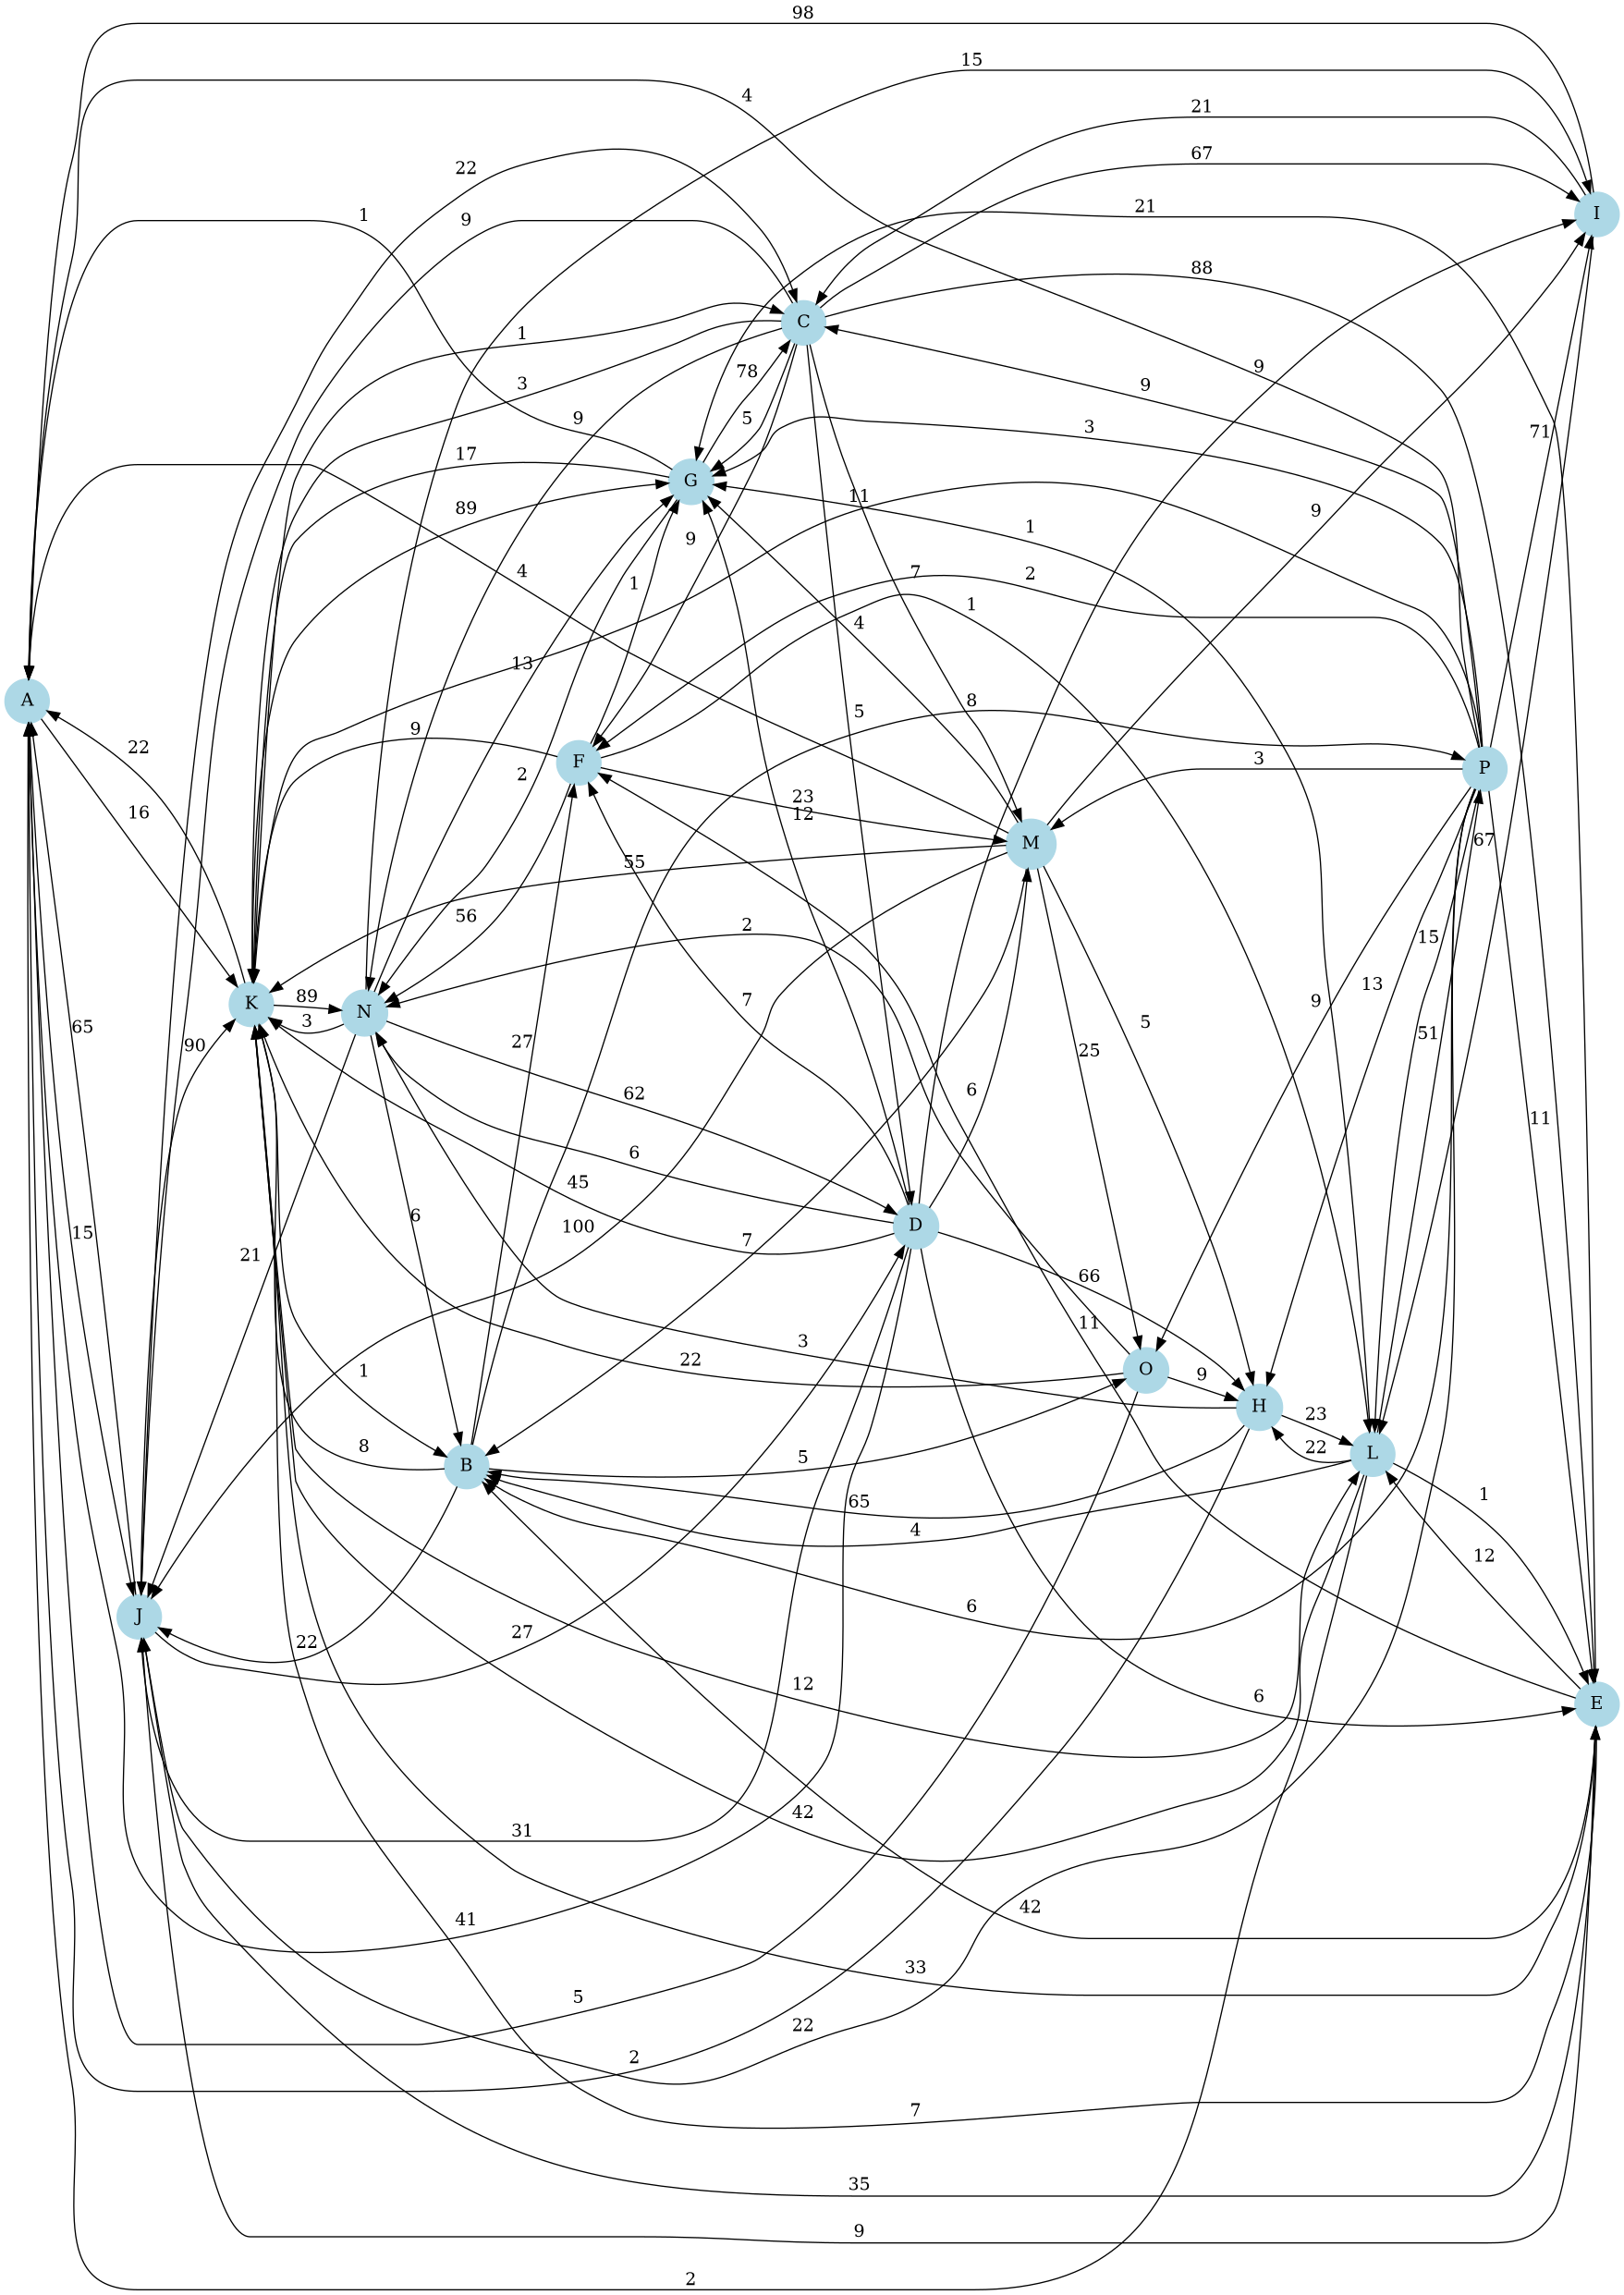
\includegraphics[width=0.5\textwidth,keepaspectratio]{grafo.png}
\caption{Representación del grafo original}
\end{figure}

\clearpage
\section{Procedimiento del Algoritmo}
\subsection{Matriz de Distancias Inicial D(0)}
\begin{table}[h!]
\centering
\begin{tabular}{|c|c|c|c|c|c|}
\hline
 & A & B & C & D & E \\\hline
A & 0 & $\infty$ & $\infty$ & $\infty$ & 6 \\\hline
B & $\infty$ & 0 & 1 & 5 & 4 \\\hline
C & 15 & $\infty$ & 0 & 21 & 23 \\\hline
D & 7 & 9 & 20 & 0 & $\infty$ \\\hline
E & $\infty$ & 8 & $\infty$ & 2 & 0 \\\hline
\end{tabular}
\caption{Matriz de distancias inicial D(0)}
\end{table}

\clearpage
\subsection{Matriz de Caminos Inicial P(0)}
\begin{table}[h!]
\centering
\begin{tabular}{|c|c|c|c|c|c|}
\hline
 & A & B & C & D & E \\\hline
A & - & - & - & - & A \\\hline
B & - & - & B & B & B \\\hline
C & C & - & - & C & C \\\hline
D & D & D & D & - & - \\\hline
E & - & E & - & E & - \\\hline
\end{tabular}
\caption{Matriz de caminos inicial P(0)}
\end{table}

\clearpage
\subsection{Iteraciones del Algoritmo}
\subsubsection{Iteración 1 (k = 1) - Nodo intermedio: A}
\begin{table}[h!]
\centering
\begin{tabular}{|c|c|c|c|c|c|}
\hline
 & A & B & C & D & E \\\hline
A & 0 & $\infty$ & $\infty$ & $\infty$ & 6 \\\hline
B & $\infty$ & 0 & 1 & 5 & 4 \\\hline
C & 15 & $\infty$ & 0 & 21 & \cellcolor{lightgreen} 21 \\\hline
D & 7 & 9 & 20 & 0 & \cellcolor{lightgreen} 13 \\\hline
E & $\infty$ & 8 & $\infty$ & 2 & 0 \\\hline
\end{tabular}
\caption{Matriz de distancias D(1) - Cambios resaltados en verde}
\end{table}

\begin{table}[h!]
\centering
\begin{tabular}{|c|c|c|c|c|c|}
\hline
 & A & B & C & D & E \\\hline
A & - & - & - & - & A \\\hline
B & - & - & B & B & B \\\hline
C & C & - & - & C & \cellcolor{lightblue} A \\\hline
D & D & D & D & - & \cellcolor{lightblue} A \\\hline
E & - & E & - & E & - \\\hline
\end{tabular}
\caption{Matriz de caminos P(1) - Cambios resaltados en azul}
\end{table}

\subsubsection{Iteración 2 (k = 2) - Nodo intermedio: B}
\begin{table}[h!]
\centering
\begin{tabular}{|c|c|c|c|c|c|}
\hline
 & A & B & C & D & E \\\hline
A & 0 & $\infty$ & $\infty$ & $\infty$ & 6 \\\hline
B & $\infty$ & 0 & 1 & 5 & 4 \\\hline
C & 15 & $\infty$ & 0 & 21 & 21 \\\hline
D & 7 & 9 & \cellcolor{lightgreen} 10 & 0 & 13 \\\hline
E & $\infty$ & 8 & \cellcolor{lightgreen} 9 & 2 & 0 \\\hline
\end{tabular}
\caption{Matriz de distancias D(2) - Cambios resaltados en verde}
\end{table}

\begin{table}[h!]
\centering
\begin{tabular}{|c|c|c|c|c|c|}
\hline
 & A & B & C & D & E \\\hline
A & - & - & - & - & A \\\hline
B & - & - & B & B & B \\\hline
C & C & - & - & C & A \\\hline
D & D & D & \cellcolor{lightblue} B & - & A \\\hline
E & - & E & \cellcolor{lightblue} B & E & - \\\hline
\end{tabular}
\caption{Matriz de caminos P(2) - Cambios resaltados en azul}
\end{table}

\subsubsection{Iteración 3 (k = 3) - Nodo intermedio: C}
\begin{table}[h!]
\centering
\begin{tabular}{|c|c|c|c|c|c|}
\hline
 & A & B & C & D & E \\\hline
A & 0 & $\infty$ & $\infty$ & $\infty$ & 6 \\\hline
B & \cellcolor{lightgreen} 16 & 0 & 1 & 5 & 4 \\\hline
C & 15 & $\infty$ & 0 & 21 & 21 \\\hline
D & 7 & 9 & 10 & 0 & 13 \\\hline
E & \cellcolor{lightgreen} 24 & 8 & 9 & 2 & 0 \\\hline
\end{tabular}
\caption{Matriz de distancias D(3) - Cambios resaltados en verde}
\end{table}

\begin{table}[h!]
\centering
\begin{tabular}{|c|c|c|c|c|c|}
\hline
 & A & B & C & D & E \\\hline
A & - & - & - & - & A \\\hline
B & \cellcolor{lightblue} C & - & B & B & B \\\hline
C & C & - & - & C & A \\\hline
D & D & D & B & - & A \\\hline
E & \cellcolor{lightblue} C & E & B & E & - \\\hline
\end{tabular}
\caption{Matriz de caminos P(3) - Cambios resaltados en azul}
\end{table}

\subsubsection{Iteración 4 (k = 4) - Nodo intermedio: D}
\begin{table}[h!]
\centering
\begin{tabular}{|c|c|c|c|c|c|}
\hline
 & A & B & C & D & E \\\hline
A & 0 & $\infty$ & $\infty$ & $\infty$ & 6 \\\hline
B & \cellcolor{lightgreen} 12 & 0 & 1 & 5 & 4 \\\hline
C & 15 & \cellcolor{lightgreen} 30 & 0 & 21 & 21 \\\hline
D & 7 & 9 & 10 & 0 & 13 \\\hline
E & \cellcolor{lightgreen} 9 & 8 & 9 & 2 & 0 \\\hline
\end{tabular}
\caption{Matriz de distancias D(4) - Cambios resaltados en verde}
\end{table}

\begin{table}[h!]
\centering
\begin{tabular}{|c|c|c|c|c|c|}
\hline
 & A & B & C & D & E \\\hline
A & - & - & - & - & A \\\hline
B & \cellcolor{lightblue} D & - & B & B & B \\\hline
C & C & \cellcolor{lightblue} D & - & C & A \\\hline
D & D & D & B & - & A \\\hline
E & \cellcolor{lightblue} D & E & B & E & - \\\hline
\end{tabular}
\caption{Matriz de caminos P(4) - Cambios resaltados en azul}
\end{table}

\subsubsection{Iteración 5 (k = 5) - Nodo intermedio: E}
\begin{table}[h!]
\centering
\begin{tabular}{|c|c|c|c|c|c|}
\hline
 & A & B & C & D & E \\\hline
A & 0 & \cellcolor{lightgreen} 14 & \cellcolor{lightgreen} 15 & \cellcolor{lightgreen} 8 & 6 \\\hline
B & 12 & 0 & 1 & 5 & 4 \\\hline
C & 15 & \cellcolor{lightgreen} 29 & 0 & 21 & 21 \\\hline
D & 7 & 9 & 10 & 0 & 13 \\\hline
E & 9 & 8 & 9 & 2 & 0 \\\hline
\end{tabular}
\caption{Matriz de distancias D(5) - Cambios resaltados en verde}
\end{table}

\begin{table}[h!]
\centering
\begin{tabular}{|c|c|c|c|c|c|}
\hline
 & A & B & C & D & E \\\hline
A & - & \cellcolor{lightblue} E & \cellcolor{lightblue} B & \cellcolor{lightblue} E & A \\\hline
B & D & - & B & B & B \\\hline
C & C & \cellcolor{lightblue} E & - & C & A \\\hline
D & D & D & B & - & A \\\hline
E & D & E & B & E & - \\\hline
\end{tabular}
\caption{Matriz de caminos P(5) - Cambios resaltados en azul}
\end{table}

\clearpage
\section{Resultados Finales}
\subsection{Matriz de Distancias Final D(5)}
\begin{table}[h!]
\centering
\begin{tabular}{|c|c|c|c|c|c|}
\hline
 & A & B & C & D & E \\\hline
A & 0 & 14 & 15 & 8 & 6 \\\hline
B & 12 & 0 & 1 & 5 & 4 \\\hline
C & 15 & 29 & 0 & 21 & 21 \\\hline
D & 7 & 9 & 10 & 0 & 13 \\\hline
E & 9 & 8 & 9 & 2 & 0 \\\hline
\end{tabular}
\caption{Matriz de distancias final D(5)}
\end{table}

\clearpage
\subsection{Matriz de Caminos Final P(5)}
\begin{table}[h!]
\centering
\begin{tabular}{|c|c|c|c|c|c|}
\hline
 & A & B & C & D & E \\\hline
A & - & E & B & E & A \\\hline
B & D & - & B & B & B \\\hline
C & C & E & - & C & A \\\hline
D & D & D & B & - & A \\\hline
E & D & E & B & E & - \\\hline
\end{tabular}
\caption{Matriz de caminos final P(5)}
\end{table}

\clearpage
\subsection{Rutas Óptimas}
\begin{itemize}
\item \textbf{A → B:} Distancia: 14, Ruta: A → E → B
\item \textbf{A → C:} Distancia: 15, Ruta: A → E → B → C
\item \textbf{A → D:} Distancia: 8, Ruta: A → E → D
\item \textbf{A → E:} Distancia: 6, Ruta: A → E
\item \textbf{B → A:} Distancia: 12, Ruta: B → D → A
\item \textbf{B → C:} Distancia: 1, Ruta: B → C
\item \textbf{B → D:} Distancia: 5, Ruta: B → D
\item \textbf{B → E:} Distancia: 4, Ruta: B → E
\item \textbf{C → A:} Distancia: 15, Ruta: C → A
\item \textbf{C → B:} Distancia: 29, Ruta: C → A → E → B
\item \textbf{C → D:} Distancia: 21, Ruta: C → D
\item \textbf{C → E:} Distancia: 21, Ruta: C → A → E
\item \textbf{D → A:} Distancia: 7, Ruta: D → A
\item \textbf{D → B:} Distancia: 9, Ruta: D → B
\item \textbf{D → C:} Distancia: 10, Ruta: D → B → C
\item \textbf{D → E:} Distancia: 13, Ruta: D → A → E
\item \textbf{E → A:} Distancia: 9, Ruta: E → D → A
\item \textbf{E → B:} Distancia: 8, Ruta: E → B
\item \textbf{E → C:} Distancia: 9, Ruta: E → B → C
\item \textbf{E → D:} Distancia: 2, Ruta: E → D
\end{itemize}
\end{document}
